%!TEX root = ../dokumentation.tex

\chapter{Praxis Kapitel}
\section{Einrichten der Entwicklungsumgebung}
Für den täglichen Gebrauch ist es nicht empfehlenswert Binaries als Root-User auszuführen. Um das HackRF One mit einem regulären Nutzer auf einem Linux System nutzen zu können, ist es notwendig eine entsprechende udev-Regel für das Gerät zu schreiben:

\begin{lstlisting}[caption=Erstellen einer udev-Regel, label=udev]
ATTR{idVendor}=="1d50", ATTR{idProduct}=="6089", SYMLINK+="hackrf-one-%k", MODE="660", GROUP="plugdev"
\end{lstlisting}

Die Datei mit der Regel wird unter /etc/udev/rules.d/ abgelegt. Verbindet man das Gerät nun mit dem Computer, wird ein Symlink unter /dev/ angelegt und Mitglieder der Gruppe \textit{plugdev} haben Zugriff darauf. 
Die erfolgreiche Installation kann durch das Ausführen des Kommandos \textbf{hackrf\_info} als User ohne root-Berechtigung überprüft werden:
\begin{lstlisting}[caption=Das Kommando "hackrf\_info" wird zum Test auf dem System ausgeführt, label=hackrfinfo]
hackrf_info version: git-a4c57ef
libhackrf version: git-a4c57ef (0.5)
Found HackRF
Index: 0
Serial number: 0000000000000000a06063c824237d5f
Board ID Number: 2 (HackRF One)
Firmware Version: 2017.02.1 (API:1.02)
Part ID Number: 0xa000cb3c 0x00544765
\end{lstlisting}

\section{Grundbausteine in GNU Radio Companion}
Um das HackRF One als Signalquelle zu verwenden, wird der quelloffene, von \ac{osmocom} \cite{osmocom:2018} entwickelte GNU Radio Block \textit{gr-osmosdr} \cite{gr-osmosdr:2018} benutzt.
Dieser untersützt das HackRF durch die zuvor installierte Bibliothek \textit{libhackrf}.

\begin{figure}[ht]
	\centering
	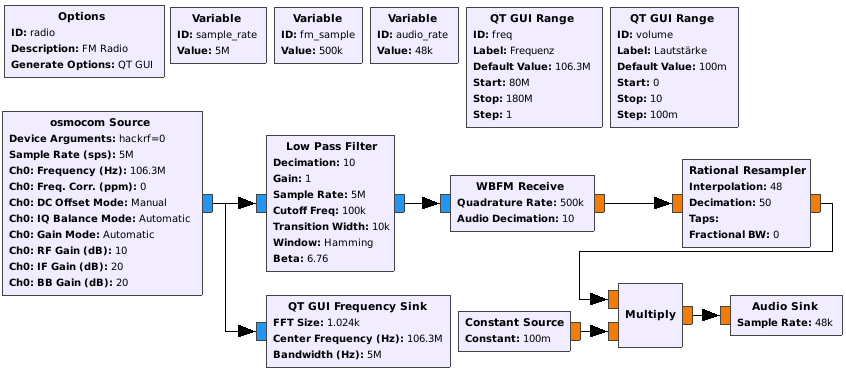
\includegraphics[width=\textwidth]{fmradio.png}
	\caption[Implementation eines FM-Radioempfängers in GNU Radio Companion]{Implementation eines FM-Radioempfängers in GNU Radio Companion. Quelle: Eigene Darstellung} 
	\label{fmradio}
\end{figure}